\chapter{Catalogazione delle debolezze}
I sistemi CVE e CVSS rappresentano un buon passo
verso la creazione di un catalogo uniforme delle
vulnerabilità. Un approccio simile è stato utilizzato anche per
l’enumerazione e la valutazione delle debolezze: il Common Weaknesses Enumeration (CWE) è un
sistema per catalogare in modo uniforme le
debolezze software. Home page: https://cwe.mitre.org. Ultima versione: 4.6 

Nelle sfide CTF che risolveremo durante il corso,
incontreremo diversi oggetti del catalogo CWE, tra cui
\begin{itemize}
    \item CWE-276: Incorrect Default Permissions
    \item CWE-272: Least Privilege Violation
    \item CWE-426: Untrusted Search Path
    \item CWE-77: Command Injection
    \item CWE-90: Authentication Bypass by Spoofing
    \item CWE-250: Execution with Unnecessary Privileges
    \item CWE-78: OS Command Injection
    \item CWE-89: SQL Injection
    \item CWE-79: Cross-site Scripting
    \item CWE-352: Cross-Site Request Forgery (CSRF)
    \item CWE-121: Stack-based Buffer Overflow 
\end{itemize}
Nelle sfide CTF che risolverete nell’ambito dei
progetti potreste incontrare altri oggetti del catalogo
CWE, tra cui:
\begin{itemize}
    \item CWE-732: Incorrect Permission Assignment for Critical
Resource
    \item CWE-59: Improper Link Resolution Before File Access
    \item CWE-261: Weak Encoding for Password
    \item CWE-257: Storing Passwords in a Recoverable Format
    \item CWE-319 : Cleartext Transmission of Sensitive Information
    \item CWE-624: Executable Regular Expression Error
    \item CWE-367: Time-Of-Check Time-Of-Use (TOCTOU) Race
Condition
    \item CWE-88: Argument Injection / Modification
    \item CWE-912: Hidden Functionality
    \item CWE-502: Deserialization of Untrusted Data
\end{itemize}

\section{Common Weaknesses Enumeration}
Il catalogo CWE è un insieme di oggetti, ciascuno
dotato di un identificatore e di un numero di attributi. Gli attributi sono: \textbf{Abstraction}, Description, Applicable platforms, Common
consequences, Likelihood of exploit, Demonstrative
examples, Potential mitigations, \textbf{Relationships}. Un oggetto può essere:
\begin{itemize}
    \item La descrizione di una singola debolezza
    \item Un elenco di identificatori a singole debolezze in
relazione tra loro
\end{itemize}
L’attributo Abstraction specifica il tipo di debolezza, e può essere di tre tipi diversi:
\begin{itemize}
    \item \textbf{Class (C)}: Debolezza descritta in termini generali, senza riferimenti
a linguaggi o tecnologie specifiche.
    \item \textbf{Base (B)}: Debolezza descritta in modo più dettagliato, in modo da
poter intuire tecniche di rilevazione e prevenzione.
    \item \textbf{Variant (V)}:Debolezza descritta nei minimi dettagli, nell’ambito di uno
specifico linguaggio e tecnologia.
\end{itemize}
L’attributo Relationships specifica il tipo di relazioni
che l’oggetto ha con altri oggetti del catalogo. Esempi di relazioni sono:
\begin{itemize}
    \item \textbf{ChildOf}: l'oggetto è figlio di un altro oggetto.
    \item \textbf{ParentOf}: l'oggetto è padre di un altro oggetto.
\end{itemize}

\begin{figure}[hbpt!]
    \centering
    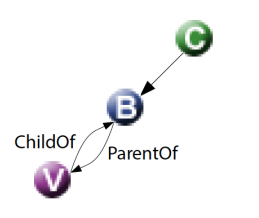
\includegraphics[width=0.3\textwidth]{./Images/cap3/3.1.png}
\end{figure}
\FloatBarrier

Un oggetto Category punta ad un insieme di oggetti
che condividono uno specifico attributo. Essendo un oggetto raggruppatore, di solito ha più
relazioni ParentOf che ChildOf:

\begin{figure}[hbpt!]
    \centering
    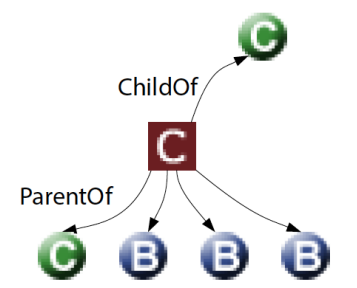
\includegraphics[width=0.3\textwidth]{./Images/cap3/3.2.png}
\end{figure}
\FloatBarrier

Un oggetto Compound mette in relazione tra loro
diverse debolezze implicate in una vulnerabilità. Ci sono due tipologie:
\begin{itemize}
    \item \textbf{Composite}: aggrega tutte le debolezze che,
sfruttate insieme, provocano
una vulnerabilità.
    \item \textbf{Chain}: aggrega tutte le debolezze che,
sfruttate in cascata, provocano
una vulnerabilità.
\end{itemize}

\section{Common Weaknesses Scoring System}
Così come per il catalogo CVE esiste il sistema di
punteggi CVSS, anche per il catalogo CWE esiste un
sistema analogo. Il Common Weaknesses Scoring System (CWSS)
è molto simile al CVSS, e ad ogni CWE id è assegnato un punteggio da 0 a 100:
\begin{itemize}
    \item 0: impatto nullo
    \item 100: conseguenze catastrofiche 
\end{itemize}
Il punteggio CWSS è dato dal prodotto di tre
sottopunteggi:
\begin{itemize}
    \item Base Finding (tra 0 e 100)
    \item Attack Surface (tra 0 e 1)
    \item Environmental (tra 0 e 1)
\end{itemize}

\begin{figure}[hbpt!]
    \centering
    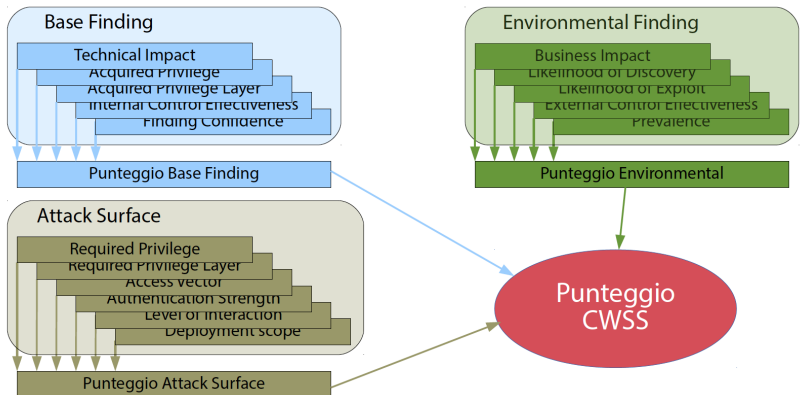
\includegraphics[width=0.7\textwidth]{./Images/cap3/3.3.png}
\end{figure}
\FloatBarrier

Ad ogni metrica è associata una domanda
a risposta multipla, e ciascuna risposta fornisce un peso numerico. I singoli pesi sono poi aggregati in un
risultato finale tramite una serie di formule.

\subsection{Metriche Base Finding}
Stimano il rischio della debolezza in sé, l’accuratezza
della scoperta, la robustezza dei meccanismi di
protezione:
\begin{itemize}
    \item E’ veramente presente? 
    \item E’ grave?
    \item E’ protetta bene?  
\end{itemize}
\subsubsection{Technical Impact}
Nell’ipotesi che la debolezza possa essere sfruttata con
successo, qual è la principale conseguenza tecnica? 
Alla metrica TI (Technical Impact) può essere
assegnato uno dei cinque valori
C (Critical), H (High), M (Medium), L (Low), N (None).

\begin{figure}[hbpt!]
    \centering
    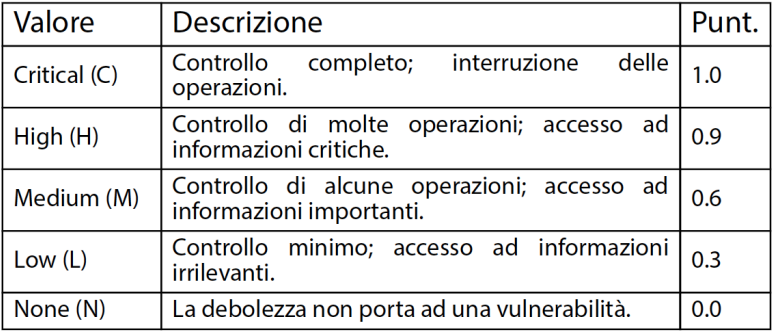
\includegraphics[width=0.4\textwidth]{./Images/cap3/3.4.png}
\end{figure}
\FloatBarrier


\subsubsection{Acquired Privilege}
Nell’ipotesi che la debolezza possa essere sfruttata con
successo, che tipi di privilegi si ottengono? Alla metrica AP (Acquired Privilege) può essere
assegnato uno dei cinque valori
A (Administrator), P (Partially Privileged User),
RU (Regular User), L (Limited or Guest), N (None).

\begin{figure}[hbpt!]
    \centering
    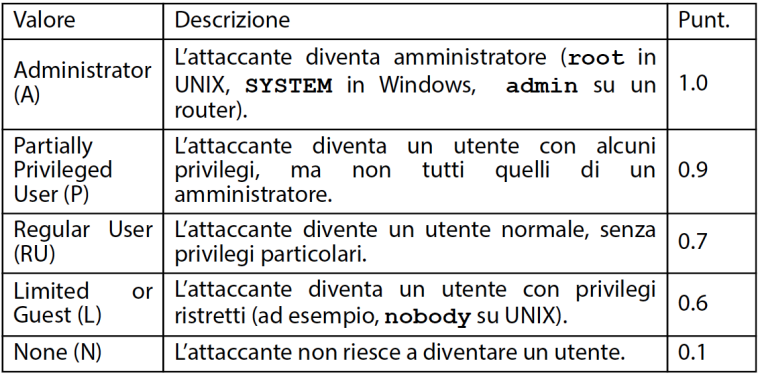
\includegraphics[width=0.4\textwidth]{./Images/cap3/3.5.png}
\end{figure}
\FloatBarrier

\subsubsection{Acquired Privilege Layer}
Nell’ipotesi che la debolezza possa essere sfruttata
con successo, a che livello operazionale
si ottengono i privilegi? Alla metrica AL (Acquired Privilege Layer) può essere
assegnato uno dei quattro valori
A (Application), S (System),
N (Network), E (Enterprise Infrastructure).

\begin{figure}[hbpt!]
    \centering
    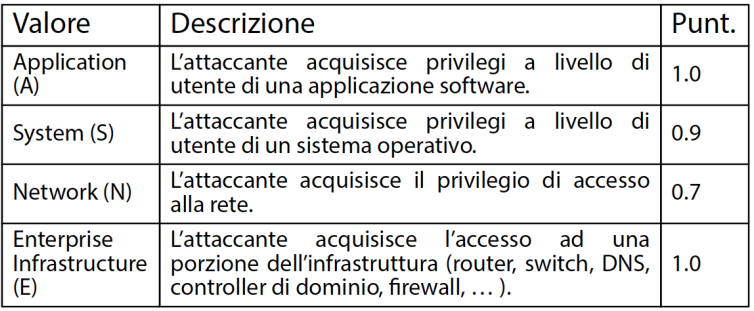
\includegraphics[width=0.4\textwidth]{./Images/cap3/3.6.png}
\end{figure}
\FloatBarrier

\subsubsection{Internal Control Effectiveness}
Qual è l’efficacia delle contromisure, a livello di codice? Alla metrica IC (Internal Control Effectiveness) può essere
assegnato uno dei sei valori
N (None), L (Limited), M (Moderate),
I (Indirect), B (Best-Available), C (Complete).

\begin{figure}[hbpt!]
    \centering
    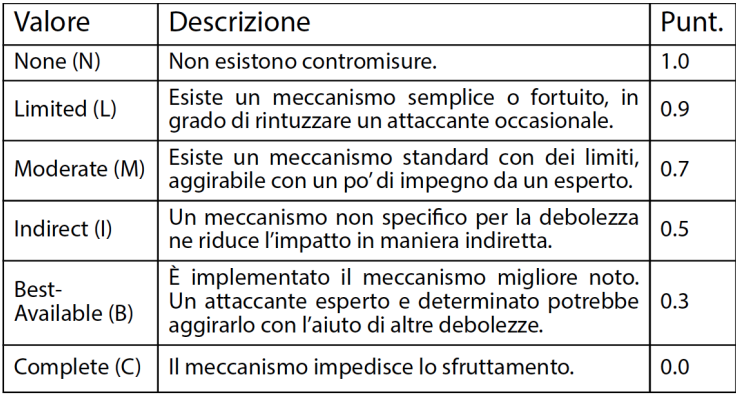
\includegraphics[width=0.4\textwidth]{./Images/cap3/3.7.png}
\end{figure}
\FloatBarrier

\subsubsection{Finding Confidence}
Quanto si è sicuri che il difetto individuato sia una
debolezza e possa essere usato da un attaccante? Alla metrica FC (Finding Confidence) può essere
assegnato uno dei tre valori
T (Proven True), LT (Proven Locally True), F (Proven False).

\begin{figure}[hbpt!]
    \centering
    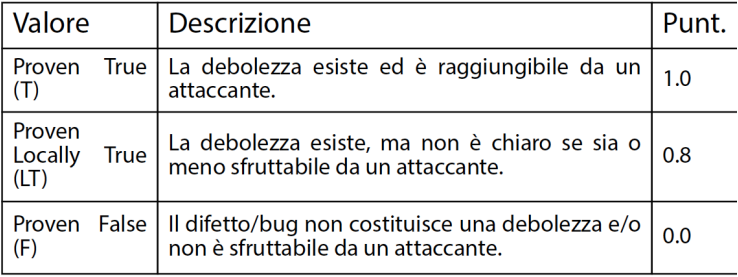
\includegraphics[width=0.4\textwidth]{./Images/cap3/3.8.png}
\end{figure}
\FloatBarrier

\subsubsection{Calcolo del Punteggio Base Findings}
Il Punteggio Base Findings è un valore tra 0 e 100,
calcolato nel modo seguente:

\[f(TI) = \begin{dcases*}
        0 & if $TI = 0$\\
        1 & otherwise. 
        \end{dcases*}
        \]
        
\[BaseFindingScore = [(10 \times TI + 5 \times(AP + AL)+5 \times FC) \times f(TI) \times IC] \times 4.0\]

\subsection{Metriche Attack Surface}
Stimano le barriere che un attaccante deve superare
per sfruttare la debolezza:
\begin{itemize}
    \item E’ necessaria l’autenticazione?
    \item Servono privilegi particolari?
\end{itemize}
\subsubsection{Required Privilege}
Quali privilegi deve già possedere l’utente
per sfruttare la debolezza? Alla metrica RP (Required Privilege) può essere
assegnato uno dei cinque valori
N (None), L (Limited or Guest), RU (Regular User),
P (Partially Privileged User), A (Administrator).

\begin{figure}[hbpt!]
    \centering
    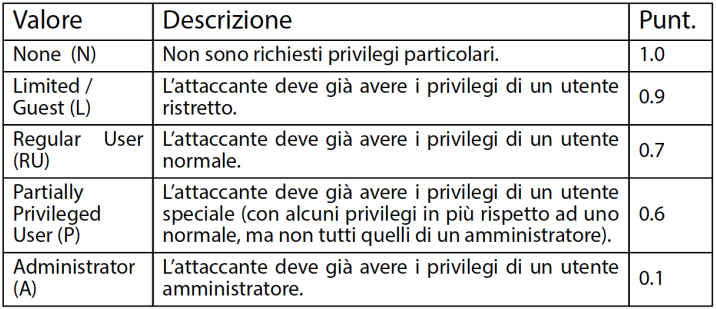
\includegraphics[width=0.4\textwidth]{./Images/cap3/3.9.png}
\end{figure}
\FloatBarrier

\subsubsection{Required Privilege Layer}
A quale livello operazionale l’attaccante deve avere
privilegi per poter sfruttare la debolezza? Alla metrica RL (Required Privilege Layer) può essere
assegnato uno dei quattro valori
A (Application), S (System), N (Network), E (Enterprise Infrastructure).

\begin{figure}[hbpt!]
    \centering
    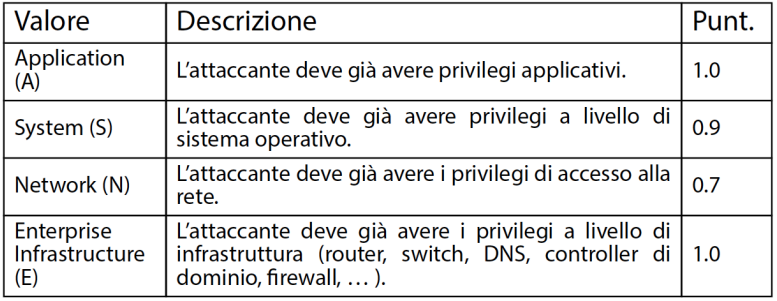
\includegraphics[width=0.4\textwidth]{./Images/cap3/3.10.png}
\end{figure}
\FloatBarrier

\subsubsection{Access Vector}
Attraverso quale canale deve comunicare l’attaccante
per poter sfruttare la debolezza? Alla metrica AV (Access Vector) può essere
assegnato uno dei sei valori
I (Internet), R (Intranet), V (Private Network),
A (Adjacent Network), L (Local), P (Physical).

\begin{figure}[hbpt!]
    \centering
    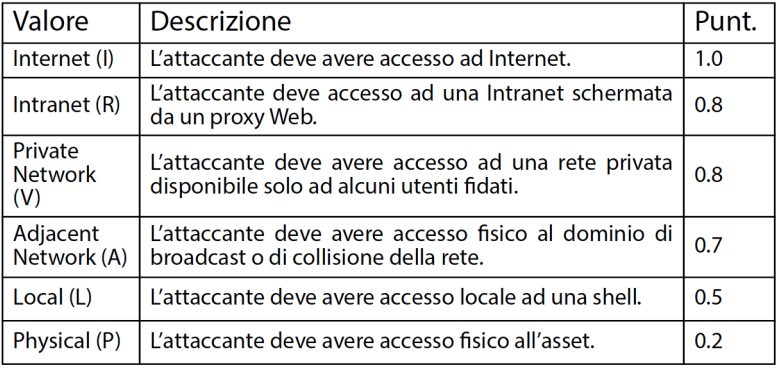
\includegraphics[width=0.4\textwidth]{./Images/cap3/3.11.png}
\end{figure}
\FloatBarrier

\subsubsection{Authentication Strength}
Quanto la procedura di autenticazione
protegge la debolezza? Alla metrica AS (Authentication Strength) può essere
assegnato uno dei quattro valori
N (None), W (Weak), M (Moderate), S (Strong).

\begin{figure}[hbpt!]
    \centering
    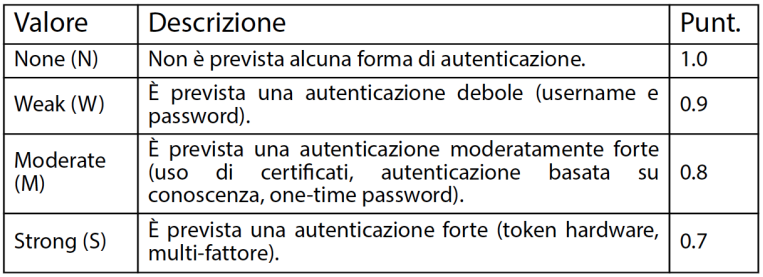
\includegraphics[width=0.4\textwidth]{./Images/cap3/3.12.png}
\end{figure}
\FloatBarrier

\subsubsection{Level of Interaction}
Quali azioni deve compiere la vittima per consentire
all’attaccante di svolgere l’attacco con successo? Alla metrica LI (Level of Interaction) può essere
assegnato uno dei sei valori
A (Automated), T (Tipical/Limited), M (Moderate),
N (OpportuNistic), H (High), NI (No Interaction).

\begin{figure}[hbpt!]
    \centering
    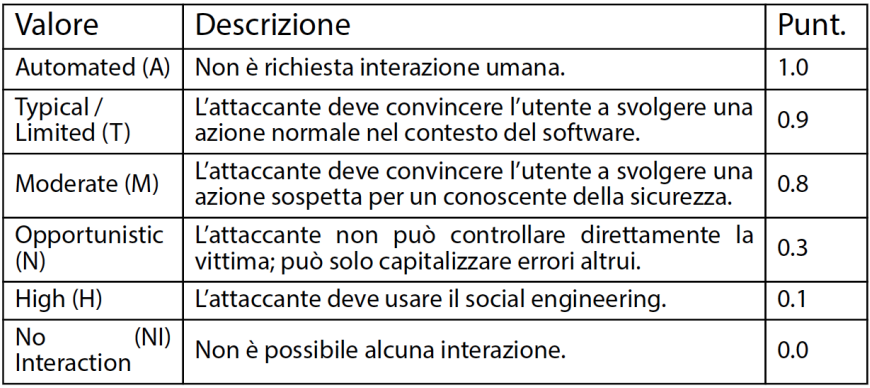
\includegraphics[width=0.4\textwidth]{./Images/cap3/3.13.png}
\end{figure}
\FloatBarrier

\subsubsection{Deployment Scope}
In quali piattaforma e/o configurazioni
si presenta la debolezza? Alla metrica DS (Deployment Scope) può essere
assegnato uno dei quattro valori
A (All), M (Moderate), R (Rare), P (Potentially Reachable).

\begin{figure}[hbpt!]
    \centering
    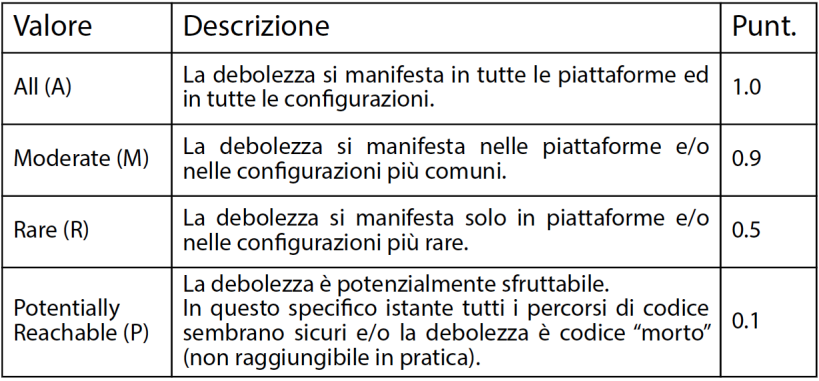
\includegraphics[width=0.4\textwidth]{./Images/cap3/3.14.png}
\end{figure}
\FloatBarrier

\subsubsection{Calcolo del Punteggio Attack Surface}
Il Punteggio Attack Surface è un valore tra 0 e 1,
calcolato nel modo seguente:

\[AttackSurfaceScore = [20 \times (RP+RL+AV)+20 \times SC + 15 \times IN \times 5 \times AS]/100.0\]

\subsection{Metriche Environmental}
Stimano le specificità legate ad uno specifico
contesto operativo:
\begin{itemize}
    \item Che impatto ha?
    \item Quanto è probabile scoprirla e usarla?
\end{itemize}

\subsubsection{Business Impact}
Qual è l’impatto ambientale di uno
sfruttamento della sicurezza? Alla metrica BI (Business Impact) può essere
assegnato uno dei cinque valori
C (Critical), H (High), M (Medium), L (Low), N (None).

\begin{figure}[hbpt!]
    \centering
    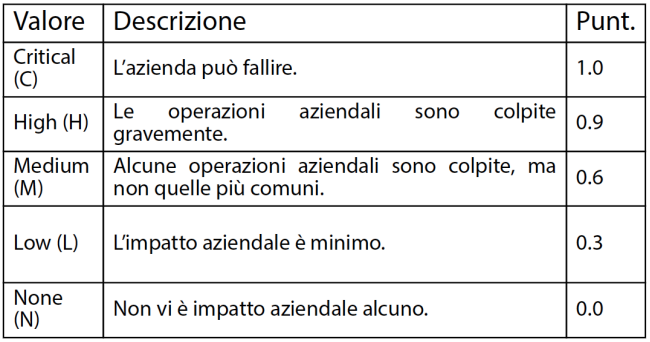
\includegraphics[width=0.4\textwidth]{./Images/cap3/3.15.png}
\end{figure}
\FloatBarrier

\subsubsection{Likelihood of Discovery}
Qual è la probabilità che un attaccante
scopra la debolezza? Alla metrica DI (Likelihood of DIscovery)
può essere assegnato uno dei tre valori
H (High), M (Medium), L (Low).

\begin{figure}[hbpt!]
    \centering
    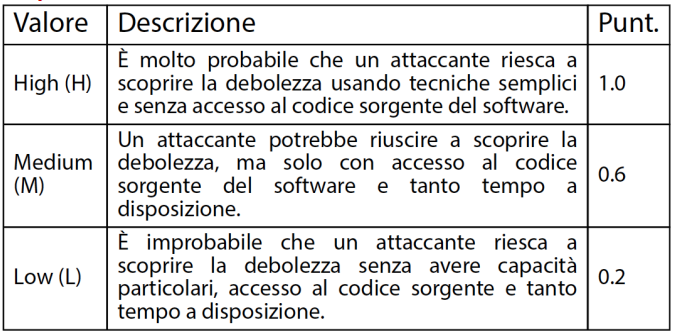
\includegraphics[width=0.4\textwidth]{./Images/cap3/3.16.png}
\end{figure}
\FloatBarrier


\subsubsection{Likelihood of Exploit}
Qual è la probabilità che, una volta scoperta la
debolezza, un attaccante con il giusto privilegio
sia in grado di sfruttarla? Alla metrica EX (Likelyhood of EXploit) può essere
assegnato uno dei quattro valori
H (High), M (Medium), L (Low), N (None).

\begin{figure}[hbpt!]
    \centering
    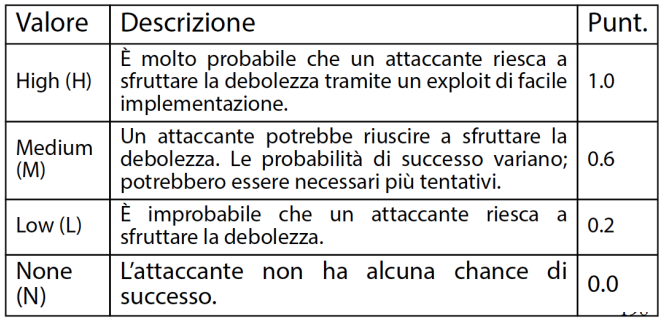
\includegraphics[width=0.4\textwidth]{./Images/cap3/3.17.png}
\end{figure}
\FloatBarrier

\subsubsection{External Control Effectiveness}
Qual è l’efficacia delle contromisure esterne
(NON a livello di codice)? Alla metrica EC (External Control Effectiveness) può essere
assegnato uno dei sei valori
N (None), L (Limited) M (Moderate),
I (Indirect), B (Best-Available), C (Complete).

\begin{figure}[hbpt!]
    \centering
    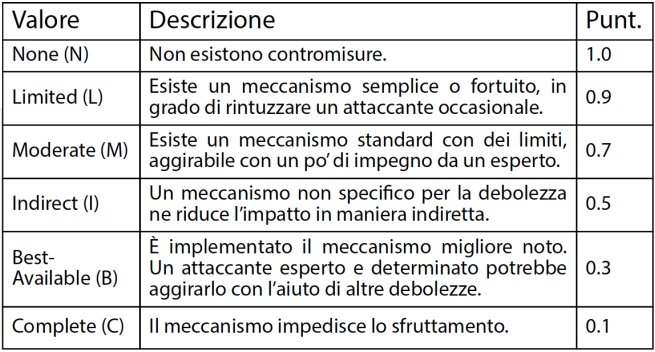
\includegraphics[width=0.4\textwidth]{./Images/cap3/3.18.png}
\end{figure}
\FloatBarrier

\subsubsection{Prevalence}
Qual è la frequenza di occorrenza della
debolezza nel software in generale? Alla metrica P (Prevalence) può essere
assegnato uno dei quattro valori
W (Widespread), H (High), C (Common), L (Limited).

\begin{figure}[hbpt!]
    \centering
    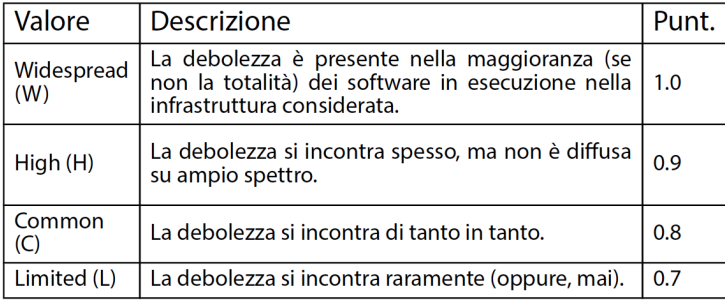
\includegraphics[width=0.4\textwidth]{./Images/cap3/3.19.png}
\end{figure}
\FloatBarrier

\subsubsection{Calcolo del Punteggio Environmental}
Il Punteggio Environmental è un valore tra 0 e 1,
calcolato nel modo seguente:

\[f(BI) = \begin{dcases*}
        0 & if $BI = 0$\\
        1 & otherwise. 
        \end{dcases*}
        \]
        
\[EnvironmentalScore = [(10 \times BI + 3 \times DI + 4 \times EX +3 \times P) \times f(BI) \times EC] \times 20.0\]

\subsubsection{Punteggio totale}
Il Punteggio Totale è un valore tra 0 e 100,
dato dal prodotto dei tre punteggi parziali. Le risposte relative alle domande del questionario sono
presentate sotto forma di stringa di testo. Tale stringa, detta \textit{vector string}, è formata da terne
di abbreviazioni domanda:risposta,peso separate dal
carattere slash. Ad esempio:
\begin{center}
    TI:H,0.9/AP:A,1.0/AL:A,1.0/IC:N,1.0/FC:T,1.0 
\end{center}

\section{Esempio di CWSS}
Si consideri un’azienda che offre i propri
prodotti al pubblico mediante un server
Web che fornisce un catalogo dei prodotti e un negozio elettronico. Una delle applicazioni utilizzate ha una debolezza: permette ad un utente di registrare un account usando
solo un indirizzo di posta elettronica. Sfruttando la debolezza, un utente può ottenere privilegi
da amministratore per l’applicazione. Si vuole calcolare il Punteggio CWSS relativo a tale
debolezza. Otteniamo maggiori dettagli sulla
debolezza:
\begin{itemize}
    \item Un attaccante non può avere controllo
completo dell’applicazione ma può cancellare
dati o utenti
    \item L’attacco non ha successo fino a quando
l’amministratore non controlla le richieste di registrazione
    \item L’applicazione non ha meccanismi di protezione della
debolezza
    \item La debolezza può essere evitata con poche righe di codice 
\end{itemize}
Iniziamo a considerare le Metriche Base Finding. Il vettore è:

\begin{center}
    TI:H,0.9/AP:A,1.0/AL:A,1.0/IC:N,1.0/FC:T,1.0
\end{center}
Punteggio Base Finding: 96.0 (vicino a 100). Il rischio legato alla debolezza è molto elevato, infatti possiamo dire che la debolezza esiste davvero e non è protetta a livello di codice. Ora consideriamo le Metriche Attack Surface. Il vettore è:
\begin{center}
     RP:L,0.9/RL:A,1.0/AV:I,1.0/AS:N,1.0/IN:T,1.0/SC:A,1.0
\end{center}
Punteggio Attack Surface: 0.965 (vicino a 1.0). Le barriere poste ad un attaccante sono poche: non sono richieste particolari credenziali e l'attacco è eseguibile da remoto. Infine consideriamo le Metriche Environmental. Il vettore è:
\begin{center}
    BI:C,0.9/DI:H,1.0/EX:H,1.0/EC:N,1.0/P:NA,1.0 
\end{center}
Punteggio Environmental: 1.0. Le condizioni ambientali sono favorevoli ad un attaccante. La debolezza è facile da scoprire e da sfruttare e non è protetta a livello operazionale (firewall, etc.).

Il punteggio CWSS è 96.0 x 0.9625 x 1.0 = 92.6

\section{Differenze tra CVSS e CWSS}
CVSS e CWSS sono molto simili, ma ci sono alcune
differenze. CVSS assume che una vulnerabilità sia già stata scoperta e
verificata, mentre CWSS può essere utilizzata prima che ciò
accada. CVSS cataloga gli errori fatti, mente CWSS cataloga gli errori
fattibili. In CVSS alcuni aspetti combinano caratteristiche multiple,
che sono invece separate in CWSS: ad esempio Access Complexity (AC) si suddivide in Required
Privilege Level e Level of Interaction.



\let\cleardoublepage\clearpage